\section{Simulation of the Shunt Active Filter Operating with an Electrohidraulic Actuator}

A simulation is proposed to evaluate the shunt active filter operating in an aircraft electrical system. The system is composed by the generation and distribution system and some loads constituted by electrohydraulic actuators with its respective shunt active filter connected to its inputs.

\subsection{Active Filter Model}

The shunt active filter model is composed by the current reference calculator and the compensator blocks. The reference calculator block is given by the procedure which uses the instantaneous power theory to define the proper reference to be applied in the compensator input. The compensator block consists of a voltage source converter (VSC), with its capacitor DC voltage regulated by a closed-loop controller. The compensator also has the hysteresis controller which creates the commands that are applied in the VSC switching devices.
The active filter operation requires a passive capacitor filter applied in the transmission lines to eliminate the high frequency content injected in the system by the switching commutation \cite{}. As the switching commutation is set at high frequency, this passive filter might be lightweight, and does not impact significantly in the aircraft system. However, the presence of capacitors in the transmission lines may decrease the power factor due to current phase shift. To eliminate this problem some inductor may be applied in the lines to compensate the reactive power flow.
The shunt active filter diagram is presented in Fig. (). This figure shows the blocks where each calculation step is accomplished, and the points where the active filter and the measurement voltage and current probes are connected.

\begin{figure*}[!b] %
	\centering
	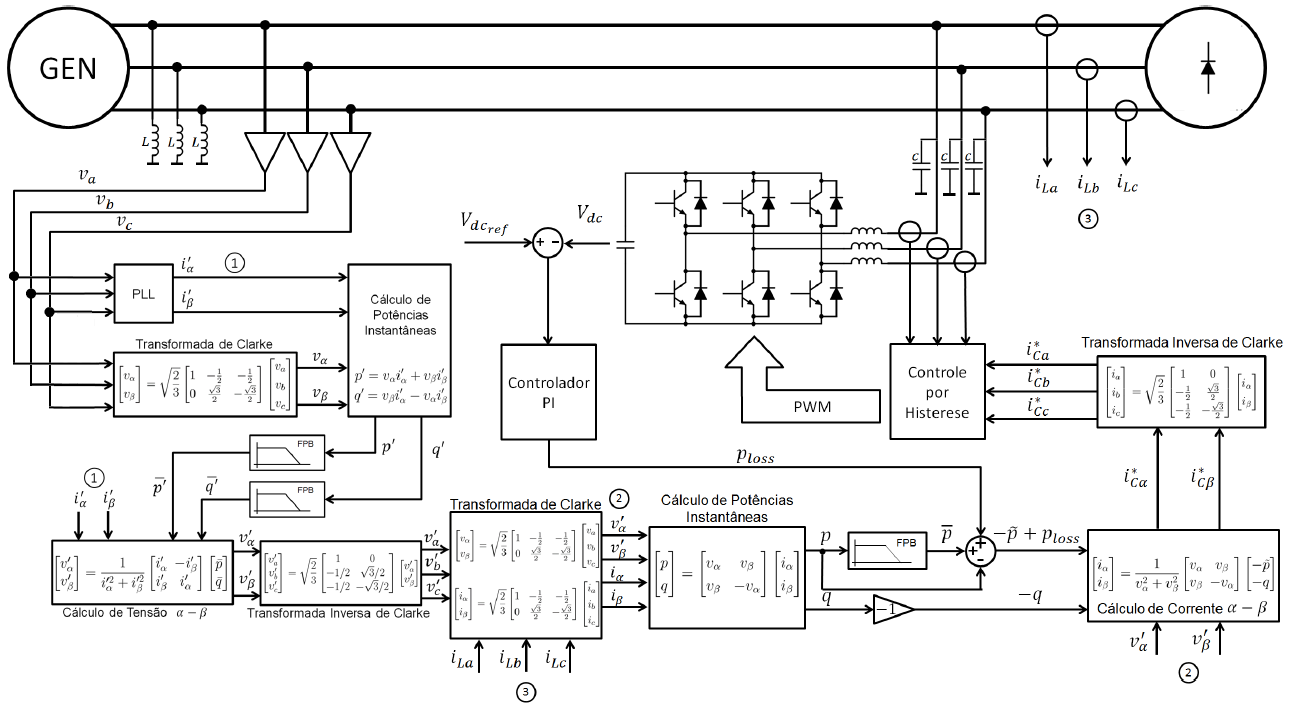
\includegraphics[width=0.85\textwidth]{Figures/filtro_blocos.png}
	\caption{}
	\label{fig:filtro_blocos.png}
\end{figure*}

\subsection{Electrical System Model}

The aircraft electrical system was modeled based on the operation of the generation and distribution system, with it respective non-idealities, which affect the power quality due to voltage drop in its terminals. The simulation presents a generator system, a power distribution system and three EHAs connected in parallel as a load.
The generator system is compound of a synchronous machine and a generator control unit (GCU). The GCU works as a field excitation controller to set the proper voltage in the PCC. The synchronous machine also has resistive and inductive reactance connected in series with the voltage source to model the resistance and the inductance presented in the generator coils.
The power distribution system is composed by the transmission lines between the generator and the PCC and between the PCC and EHAs. In the PCC, it is located the probes which measure the system voltages levels and send as the reference input to the GCU. The lines power distribution lines transmission are modeled as resistive and inductive reactance in series for each 3 phase lines.
The EHA is an equipment used in the aircraft aerodynamic surfaces for latero-directional and longitudinal control. This equipment is a non-linear load, since in its input has a 3-phase diode bridge. The EHAs modeled has a 3phase Graetz diode bridge with a current controlled source placed in its respective DC side. The controlled current source is defined to operate in such way to recreates the apparent power consumption of a real EHA. Thereby, this guarantees the distorted current waveforms generated by the EHA in real operation.

\subsection{Results}

\todo[inline]{colocar os resultados da simulação para o caso onde não há carga e para a máxima carga. Apenas curvas de forma de onda de tensão e corrente e espectro de frequência (se couber, também no período com pouca carga)}

Testes / ensaios. Deixe claro como foram realizados os ensaios, tipo de montagem, identifique possíveis problemas que interferiram nos resultados etc. 
Convença o leitor que você realizou os testes / ensaios  incluindo figuras, gráficos etc.  
Apresente os resultados e compare com trabalhos disponíveis na literatura. Discuta pontos fortes e fracos (do seu trabalho e trabalhos anteriores). Não exagere nos resultados positivos atingidos e não enfatize em demasia os pontos  negativos de outros trabalhos (o revisor do seu artigo pode ser um dos autores dos trabalhos que você está comparando).
